% !TeX root = RJwrapper.tex
\title{Variable Importance Plots---An Introduction to the \pkg{vip} Package}
\author{by Brandon M. Greenwell, Bradley C. Boehmke}

\maketitle

\abstract{%
In the era of ``big data'', it is becoming more of a challenge to not
only build state-of-the-art predictive models, but also gain an
understanding of what's really going on in the data. For example, it is
often of interest to know which, if any, of the predictors in a fitted
model are relatively influential on the predicted outcome. Some modern
algorithms---like random forests (RFs) and gradient boosted decision
trees (GBMs)---have a natural way of quantifying the importance or
relative influence of each feature. Other algorithms---like naive Bayes
classifiers and support vector machines---are not capable of doing so
and \dfn{model-agnostic approaches} are generally used to measure each
predictor's importance. Enter \pkg{vip}, an R package for constructing
variable importance scores/plots for many types of supervised learning
algorithms using model-specific and novel model-agnostic approaches.
We'll also discuss a novel way to display both feature importance and
feature effects together using \dfn{sparklines}, a very small line chart
conveying the general shape or variation in some feature that can be
directly embedded in text or tables.
}

\hypertarget{introduction}{%
\subsection{Introduction}\label{introduction}}

Too often machine learning (ML) models are summarized using a single
metric (e.g., cross-validated accuracy) and then put into production.
Although we often care about the predictions from these models, it is
becoming routine to also understand the predictions! Understanding how
an ML model makes its predictions helps build trust in the model and is
the fundamental idea of the emerging field of
\dfn{interpretable machine learning} (IML). For an in-depth discussion
on IML, see \citet{molnar-2019-iml}. In this paper, we focus on global
methods for quantifying the importance of features in an ML model.
Computing variable importance (VI) and communicating them through
variable importance plots (VIPs) is a fundamental component of IML and
is the main topic of this paper.

VI scores and VIPs can be constructed for general ML models using a
number of packages. The \CRANpkg{iml} package \citep{iml-pkg} provides
the \code{FeatureImp()} function which computes feature importance for
general prediction models using the permutation approach (discussed
later). It is written in \CRANpkg{R6} \citep{R6-pkg} and allows the user
to specify a generic loss function or select one from a pre-defined list
(e.g., \code{loss = "mse"} for mean squared error). It also allows the
user to specify whether importance is measured as the difference or as
the ratio of the original model error and the model error after
permutation. The user can also specify the number of repetitions used
when permuting each feature to help stabilize the variability in the
procedure.

The \CRANpkg{ingredients} package \citep{ingredients-pkg} also provides
permutation-based VI scores through the \code{feature\_importance()}
function. (Note that this function recently replaced the now deprecated
\CRANpkg{DALEX} function \code{variable\_importance()}
\citep{DALEX-pkg}.) Similar to \code{iml::FeatureImp()}, this function
allows the user to specify a loss function and how the importance scores
are computed (e.g., using the difference or ratio). It also provides an
option to sample the training data before shuffling the data to compute
importance (the default is to use \code{n\_sample = 1000}). This can
help speed up computation.

The \CRANpkg{caret} package \citep{caret-pkg} includes a general
\code{varImp()} function for computing model-specific and filter-based
VI scores. Filter-based approaches, which are described in
\citet{applied-kuhn-2013}, do not make use of the fitted model to
measure VI. They also do not take into account the other predictors in
the model. For regression problems, a popular filter-based approach to
measuring the VI of a numeric predictor \(x\) is to first fit a flexible
nonparametric model between \(x\) and the target \(Y\); for example, the
locally-weighted polynomial regression (LOWESS) method developed by
\citet{robust-cleveland-1979}. From this fit, a pseudo-\(R^2\) measure
can be obtained from the resulting residuals and used as a measure of
VI. For categorical predictors, a different method based on standard
statistical tests (e.g., \(t\)-tests and ANOVAs) can be employed; see
\citet{applied-kuhn-2013} for details. For classification problems, an
area under the ROC curve (AUC) statistic can be used to quantify
predictor importance. The AUC statistic is computed by using the
predictor \(x\) as input to the ROC curve. If \(x\) can reasonably
separate the classes of \(Y\), that is a clear indicator that \(x\) is
an important predictor (in terms of class separation) and this is
captured in the corresponding AUC statistic. For problems with more than
two classes, extensions of the ROC curve or a one-vs-all approach can be
used.

If you use the \CRANpkg{mlr} interface for fitting ML models
\citep{mlr-pkg}, then you can use the \code{getFeatureImportance()}
function to extract model-specific VI scores from various tree-based
models (e.g., RFs and GBMs). Unlike \pkg{caret}, the model needs to be
fit via the \pkg{mlr} interface; for instance, you cannot use
\code{getFeatureImportance()} on a \CRANpkg{gbm} model \citep{gbm-pkg}
unless it was fit using \pkg{mlr}.

While the \pkg{iml} and \pkg{DALEX} packages provide model-agnostic
approaches to computing VI, \pkg{caret}, and to some extent \pkg{mlr},
provide model-specific approaches (e.g., using the absolute value of the
\(t\)-statistic for linear models) as well less accurate filter-based
approaches . Furthermore, each package has a completely different
interface (e.g., \pkg{iml} is written in R6). The \CRANpkg{vip} package
\citep{vip-pkg} strives to provide a consistent interface to both
model-specific and model-agnostic approaches to feature importance that
is simple to use. The three most important functions exported by
\pkg{vip} are described below:

\begin{itemize}
 
  \item \code{vi()} computes VI scores using model-specific or model-agnostic approaches (the results are always returned as a tibble \citep{tibble-pkg});
  
  \item \code{vip()} constructs VIPs using model-specific or model-agnostic approaches with \CRANpkg{ggplot2}-style graphics \citep{ggplot2-pkg};
  
  \item \code{add\_sparklines()} adds a novel sparkline representation of feature effects (e.g., \dfn{partial dependence plots}) to any VI table produced by \code{vi()}.

\end{itemize}

There's also a function called \code{vint()} (for variable interactions)
but is experimental and will not be discussed here; the interested
reader is pointed to \citet{greenwell-simple-2018}. Note that
\code{vi()} is actually a wrapper around four workhorse functions,
\code{vi\_model()}, \code{vi\_ice()}, \code{vi\_pdp()}, and
\code{vi\_permute()}, that compute various types of VI scores. The first
computes model-specific VI scores, while the latter three produce
model-agnostic ones. The workhorse function that actually gets called is
controlled by the \code{method} argument in \code{vi()}; the default is
\code{method = "model"} which corresponds to model-specific VI (see
\code{?vip::vi} for details and links to further documentation).

\hypertarget{constructing-vips-in-r}{%
\subsection{Constructing VIPs in R}\label{constructing-vips-in-r}}

We'll illustrate major concepts using the Friedman 1 benchmark problem
described in \citet{multivariate-friedman-1991} and
\citet{bagging-breiman-1996}:

\begin{equation}
  Y_i = 10 \sin\left(\pi X_{1i} X_{2i}\right) + 20 \left(X_{3i} - 0.5\right) ^ 2 + 10 X_{4i} + 5 X_{5i} + \epsilon_i, \quad i = 1, 2, \dots, n,
\label{eqn:friedman1}
\end{equation}

where \(\epsilon_i \stackrel{iid}{\sim} N\left(0, \sigma^2\right)\).
Data from this model can be generated using the
\code{vip::gen\_friedman()}. By default, the features consist of 10
independent variables uniformly distributed on the interval
\(\left[0,1\right]\); however, only 5 out of these 10 are actually used
in the true model. The code chunk below simulates 500 observations from
the model in Equation\textasciitilde{}\eqref{eqn:friedman1} with
\(\sigma = 1\); see \code{?vip::gen\_friedman} for details.

\begin{Schunk}
\begin{Sinput}
trn <- vip::gen_friedman(500, sigma = 1, seed = 101)  # simulate training data
tibble::as_tibble(trn)  # inspect output
\end{Sinput}
\begin{Soutput}
#> # A tibble: 500 x 11
#>        y     x1    x2    x3    x4     x5      x6    x7    x8    x9   x10
#>    <dbl>  <dbl> <dbl> <dbl> <dbl>  <dbl>   <dbl> <dbl> <dbl> <dbl> <dbl>
#>  1 14.9  0.372  0.406 0.102 0.322 0.693  0.758   0.518 0.530 0.878 0.763
#>  2 15.3  0.0438 0.602 0.602 0.999 0.776  0.533   0.509 0.487 0.118 0.176
#>  3 15.1  0.710  0.362 0.254 0.548 0.0180 0.765   0.715 0.844 0.334 0.118
#>  4 10.7  0.658  0.291 0.542 0.327 0.230  0.301   0.177 0.346 0.474 0.283
#>  5 17.6  0.250  0.794 0.383 0.947 0.462  0.00487 0.270 0.114 0.489 0.311
#>  6 18.3  0.300  0.701 0.992 0.386 0.666  0.198   0.924 0.775 0.736 0.974
#>  7 14.6  0.585  0.365 0.283 0.488 0.845  0.466   0.715 0.202 0.905 0.640
#>  8 17.0  0.333  0.552 0.858 0.509 0.697  0.388   0.260 0.355 0.517 0.165
#>  9  8.54 0.622  0.118 0.490 0.390 0.468  0.360   0.572 0.891 0.682 0.717
#> 10 15.0  0.546  0.150 0.476 0.706 0.829  0.373   0.192 0.873 0.456 0.694
#> # ... with 490 more rows
\end{Soutput}
\end{Schunk}

From Equation\textasciitilde{}\eqref{eqn:friedman1}, it should be clear
that features \(X_1\)--\(X_5\) are the most important! (The others don't
influence \(Y\) at all.) Also, based on the form of the model, we'd
expect \(X_4\) to be the most important feature, probably followed by
\(X_1\) and \(X_2\) (both comparably important), with \(X_5\) probably
less important. The influence of \(X_3\) is harder to determine due to
its quadratic nature, but it seems likely that this nonlinearity will
suppress the variable's influence over its observed range (i.e., 0--1).

\section{Model-specific VI}

Some machine learning algorithms have their own way of quantifying the
importance of each feature. We describe some of these in the subsections
that follow. The issue with model-specific VI scores is that they are
not necessarily comparable across different types of models. For
example, directly comparing the impurity-based VI scores from tree-based
models to the \(t\)-statistic from linear models.

\subsection{Decision trees and tree ensembles}

Decision trees probably offer the most natural model-specific approach
to quantifying the importance of each feature. In a binary decision
tree, at each node \(t\), a single predictor is used to partition the
data into two homogeneous groups. The chosen predictor is the one that
maximizes some measure of improvement \(i^t\). The relative importance
of predictor \(X\) is the sum of the squared improvements over all
internal nodes of the tree for which \(X\) was chosen as the
partitioning variable; see \citet{classification-breiman-1984} for
details. This idea also extends to ensembles of decision trees, such as
RFs and GBMs. In ensembles, the improvement score for each predictor is
averaged across all the trees in the ensemble. Fortunately, due to the
stabilizing effect of averaging, the improvement-based VI metric is
often more reliable in large ensembles; see
\citet[p. 368]{hastie-elements-2009}. RFs offer an additional method for
computing VI scores. The idea is to use the leftover out-of-bag (OOB)
data to construct validation-set errors for each tree. Then, each
predictor is randomly shuffled in the OOB data and the error is computed
again. The idea is that if variable \(X\) is important, then the
validation error will go up when \(X\) is perturbed in the OOB data. The
difference in the two errors is recorded for the OOB data then averaged
across all trees in the forest. Later on, we'll discuss a more general
permutation method that can be applied to any supervised learning model.

To illustrate, we fit a CART-like regression tree, RF, and GBM to the
simulated training data. (Note: there are a number of different packages
available for fitting these types of models, we just picked popular
implementations for illustration.)

\begin{Schunk}
\begin{Sinput}
# Load required packages
library(rpart)          # for fitting CART-like decision trees
library(randomForest)   # for fitting RFs
library(xgboost)        # for fitting GBMs

# Fit a single regression tree
tree <- rpart(y ~ ., data = trn)

# Fit an RF
set.seed(101)
rfo <- randomForest(y ~ ., data = trn, importance = TRUE)

# Fit a GBM
set.seed(102)
bst <- xgboost(
  data = data.matrix(subset(trn, select = -y)),
  label = trn$y, 
  objective = "reg:linear",
  nrounds = 100, 
  max_depth = 5, 
  eta = 0.3,
  verbose = 0  # suppress printing
)
\end{Sinput}
\end{Schunk}

Each of the above packages include the ability to compute VI scores for
all the features in the model; however, the implementation is rather
package specific, as shown in the code chunk below. The results are
displayed in Figure\textasciitilde{}\ref{fig:vi-plots} (the code to
reproduce these plots has been omitted but can be made available upon
request).

\begin{Schunk}
\begin{Sinput}
# Extract VI scores from each model
vi_tree <- tree$variable.importance
vi_rfo <- rfo$variable.importance
vi_bst <- xgb.importance(model = bst)
\end{Sinput}
\end{Schunk}

\begin{Schunk}
\begin{figure}

{\centering 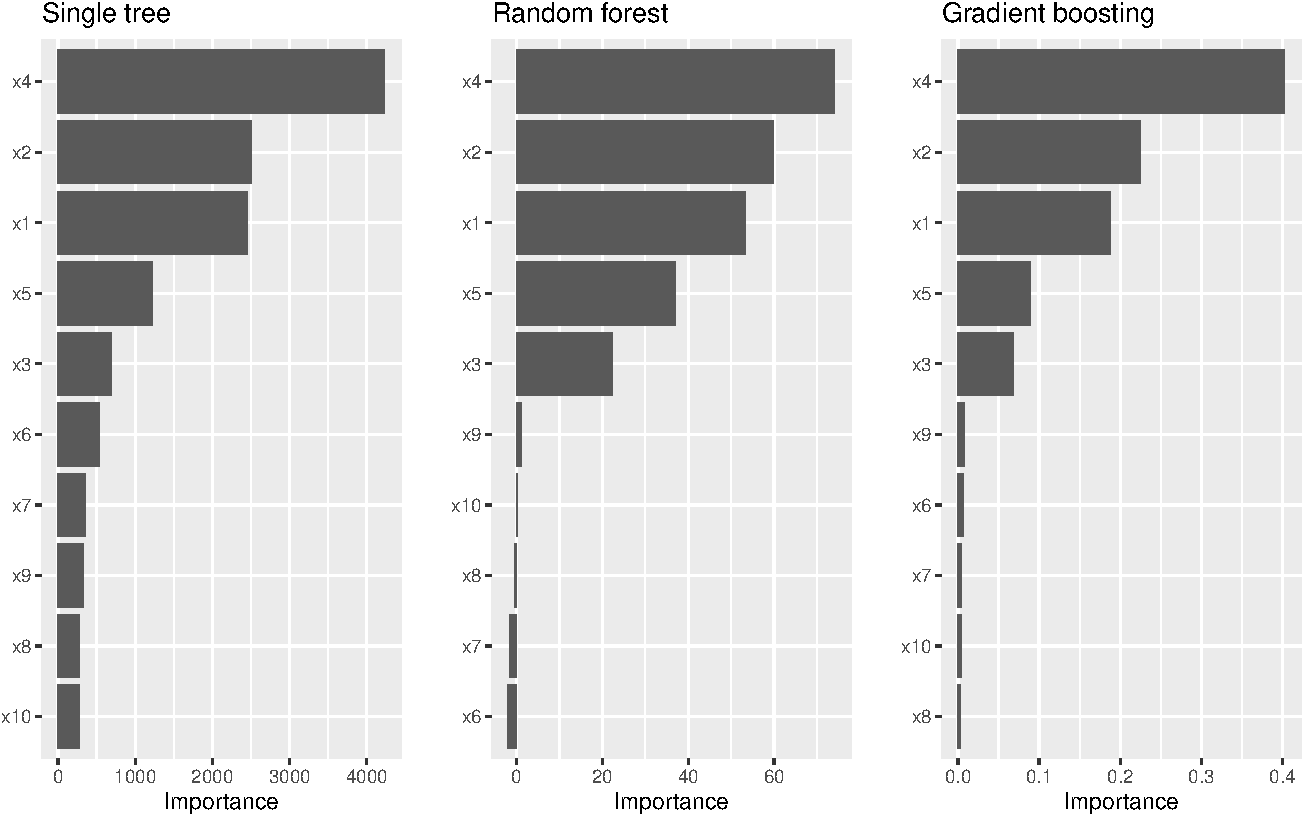
\includegraphics[width=1\linewidth]{greenwell-boehmke_files/figure-latex/vi-plots-1} 

}

\caption[Model-specific VIPs for the three different tree-based models fit to the simulated Friedman data]{Model-specific VIPs for the three different tree-based models fit to the simulated Friedman data.}\label{fig:vi-plots}
\end{figure}
\end{Schunk}

As we would expect, all three methods rank the variables
\code{x1}--\code{x5} as more important than the others. While this is
good news, it is unfortunate that we have to remember the different
functions and ways of extracting and plotting VI scores from various
model fitting functions. This is one place where \pkg{vip} can
help\ldots{}one function to rule them all! Once \pkg{vip} is loaded, we
can use \code{vi()} to extract a tibble of VI scores.

\begin{Schunk}
\begin{Sinput}
# Load required packages
library(vip)

# Compute model-specific VI scores
vi(tree)  # CART-like decision tree
\end{Sinput}
\begin{Soutput}
#> # A tibble: 10 x 2
#>    Variable Importance
#>    <chr>         <dbl>
#>  1 x4            4234.
#>  2 x2            2513.
#>  3 x1            2461.
#>  4 x5            1230.
#>  5 x3             688.
#>  6 x6             533.
#>  7 x7             357.
#>  8 x9             331.
#>  9 x8             276.
#> 10 x10            275.
\end{Soutput}
\begin{Sinput}
vi(rfo)   # RF
\end{Sinput}
\begin{Soutput}
#> # A tibble: 10 x 2
#>    Variable Importance
#>    <chr>         <dbl>
#>  1 x4           74.2  
#>  2 x2           59.9  
#>  3 x1           53.3  
#>  4 x5           37.1  
#>  5 x3           22.5  
#>  6 x9            1.05 
#>  7 x10           0.254
#>  8 x8           -0.408
#>  9 x7           -1.56 
#> 10 x6           -2.00
\end{Soutput}
\begin{Sinput}
vi(bst)   # GBM
\end{Sinput}
\begin{Soutput}
#> # A tibble: 10 x 2
#>    Variable Importance
#>    <chr>         <dbl>
#>  1 x4          0.403  
#>  2 x2          0.225  
#>  3 x1          0.189  
#>  4 x5          0.0894 
#>  5 x3          0.0682 
#>  6 x9          0.00802
#>  7 x6          0.00746
#>  8 x7          0.00400
#>  9 x10         0.00377
#> 10 x8          0.00262
\end{Soutput}
\end{Schunk}

Notice how the \code{vi()} function always returns a
tibble\footnote{Technically, it's a tibble with an additional \code{"vi"} class.}
with two columns: \code{Variable} and \code{Importance} (the exceptions
are coefficient-based models which also include a \code{Sign} column
giving the sign of the corresponding coefficient and permutation
importance involving multiple Monte Carlo simulations, but more on that
later). Also, by default, \code{vi()} always orders the VI scores from
highest to lowest; this, among other options, can be controlled by the
user (see \code{?vip::vi} for details). Plotting VI scores with
\code{vip()} is just as straightforward. For example, the following code
can be used to reproduce Figure\textasciitilde{}\ref{fig:vi-plots}.

\begin{Schunk}
\begin{Sinput}
p1 <- vip(tree) + ggtitle("Single tree")
p2 <- vip(rfo) + ggtitle("Random forest")
p3 <- vip(bst) + ggtitle("Gradient boosting")

# Figure 1
grid.arrange(p1, p2, p3, nrow = 1)
\end{Sinput}
\end{Schunk}

Notice how the \code{vip()} function always returns a \code{"ggplot"}
object (by default, this will be a bar plot). For large models with many
features, a Cleveland dot plot is more effective (in fact, a number of
useful plotting options can be fiddled with). Below we call \code{vip()}
and change a few useful options (the resulting plot is displayed in
Figure\textasciitilde{}\ref{fig:dot-plot}). Note that we can also call
\code{vip()} directly on a \code{"vi"} objects if it's already been
constructed.

\begin{Schunk}
\begin{Sinput}
# Load required packages
library(ggplot2)  # for theme_light() function
theme_set(theme_light())  # set theme for all ggplot2-based plots

vip(bst, num_features = 5, geom = "point", horizontal = FALSE, 
    aesthetics = list(color = "red", shape = 17, size = 4)) 
\end{Sinput}
\begin{figure}

{\centering 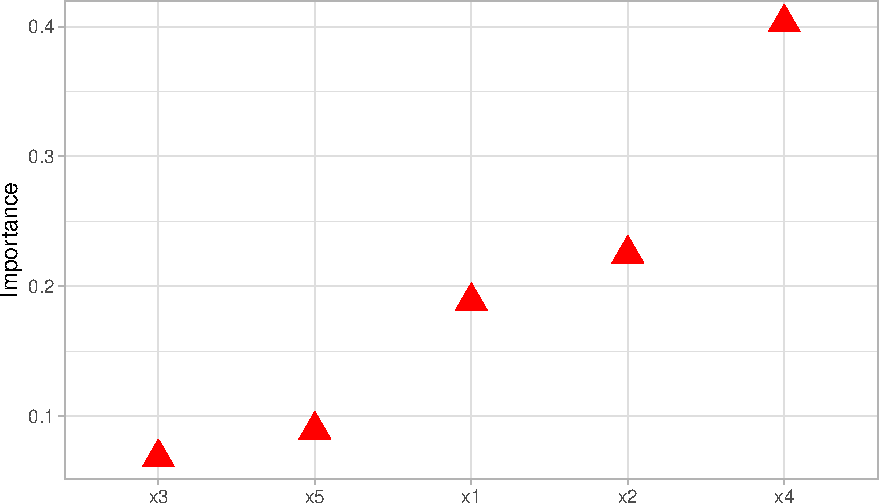
\includegraphics[width=0.7\linewidth]{greenwell-boehmke_files/figure-latex/dot-plot-1} 

}

\caption[Illustrating various plotting options]{Illustrating various plotting options.}\label{fig:dot-plot}
\end{figure}
\end{Schunk}

\hypertarget{linear-models}{%
\subsection{Linear models}\label{linear-models}}

In multiple linear regression, or linear models (LMs), the absolute
value of the \(t\)-statistic (or some other scaled variant of the
estimated coefficients) is commonly used as a measure of VI. The same
idea also extends to generalized linear models (GLMs). In the code chunk
below, we fit an LM to the simulated \code{trn} data set allowing for
all main effects and two-way interactions, then use the \code{step()}
function to perform backward elimination. The resulting VIP is displayed
in Figure\textasciitilde{}\ref{fig:vip-step}.

\begin{Schunk}
\begin{Sinput}
# Fit a LM
linmod <- lm(y ~ .^2, data = trn)
backward <- step(linmod, direction = "backward", trace = 0)

# Extract VI scores
(vi_backward <- vi(backward))
\end{Sinput}
\begin{Soutput}
#> # A tibble: 21 x 3
#>    Variable Importance Sign 
#>    <chr>         <dbl> <chr>
#>  1 x4            14.2  POS  
#>  2 x2             7.31 POS  
#>  3 x1             5.63 POS  
#>  4 x5             5.21 POS  
#>  5 x3:x5          2.46 POS  
#>  6 x1:x10         2.41 NEG  
#>  7 x2:x6          2.41 NEG  
#>  8 x1:x5          2.37 NEG  
#>  9 x10            2.21 POS  
#> 10 x3:x4          2.01 NEG  
#> # ... with 11 more rows
\end{Soutput}
\begin{Sinput}
# Plot VI scores; by default, `vip()` displays the top ten features
vip(vi_backward, num_features = length(coef(backward)), 
    geom = "point", horizontal = FALSE)
\end{Sinput}
\begin{figure}

{\centering 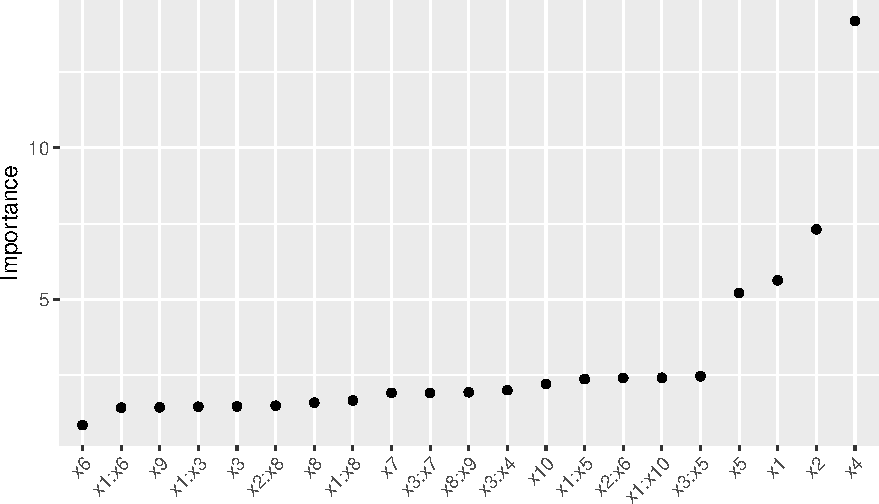
\includegraphics[width=0.7\linewidth]{greenwell-boehmke_files/figure-latex/vip-step-1} 

}

\caption[Example VIP from a linear model fit to the simulated Friedman data]{Example VIP from a linear model fit to the simulated Friedman data.}\label{fig:vip-step}
\end{figure}
\end{Schunk}

One issue with computing VI scores for LMs using the \(t\)-statistic
approach is that a score is assigned to each term in the model, rather
than to each individual feature! We can solve this problem using one of
the model-agnostic approaches discussed later.

Multivariate adaptive regression splines (MARS), which were introduced
in \citet{multivariate-friedman-1991}, is an automatic regression
technique and can be seen as a generalization of LMs and GLMs. In the
MARS algorithm, the contribution (or VI score) for each predictor is
determined using a generalized cross-validation (GCV) statistic (though,
other statistics can also be used; see \code{?vip::vi\_model} for
details). An example using the \CRANpkg{earth} package \citep{earth-pkg}
is given below (the results are plotted in
Figure\textasciitilde{}\ref{fig:vip-earth}):

\begin{Schunk}
\begin{Sinput}
# Load required packages
library(earth)

# Fit a MARS model
mars <- earth(y ~ ., data = trn, degree = 2, pmethod = "exhaustive")

# Extract VI scores
vi(mars, type = "gcv")
\end{Sinput}
\begin{Soutput}
#> # A tibble: 10 x 2
#>    Variable Importance
#>    <chr>         <dbl>
#>  1 x4            100  
#>  2 x1             83.2
#>  3 x2             83.2
#>  4 x5             59.3
#>  5 x3             43.5
#>  6 x6              0  
#>  7 x7              0  
#>  8 x8              0  
#>  9 x9              0  
#> 10 x10             0
\end{Soutput}
\begin{Sinput}
# Plot VI scores
vip(mars)
\end{Sinput}
\begin{figure}

{\centering 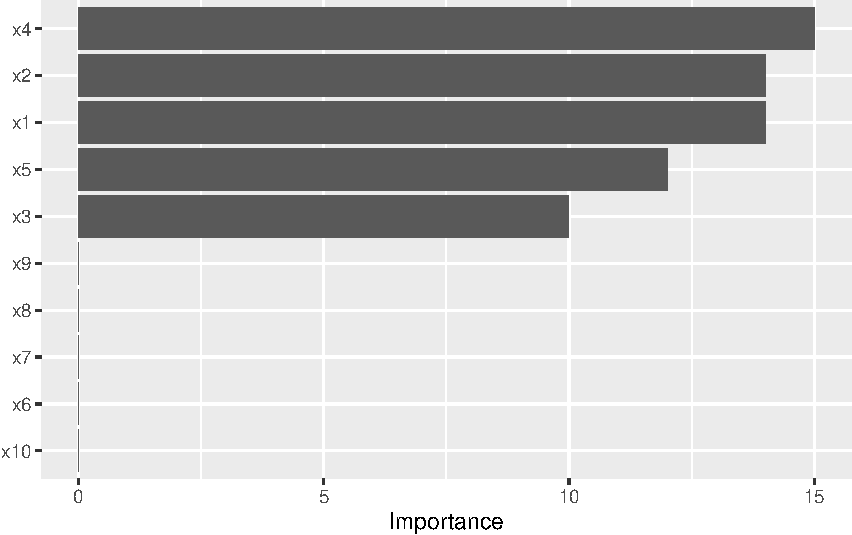
\includegraphics[width=0.7\linewidth]{greenwell-boehmke_files/figure-latex/vip-earth-1} 

}

\caption[Example VIP from a MARS model fit to the simulated Friedman data]{Example VIP from a MARS model fit to the simulated Friedman data.}\label{fig:vip-earth}
\end{figure}
\end{Schunk}

To access VI scores directly in \pkg{earth}, you can use the
\code{earth::evimp()} function.

\hypertarget{neural-networks}{%
\subsection{Neural networks}\label{neural-networks}}

For neural netwroks (NNs), two popular methods for constructing VI
scores are the Garson algorithm \citep{interpreting-garson-1991}, later
modified by \citet{back-goh-1995}, and the Olden algorithm
\citep{accurate-olden-2004}. For both algorithms, the basis of these VI
scores is the network's connection weights. The Garson algorithm
determines VI by identifying all weighted connections between the nodes
of interest. Olden's algorithm, on the other hand, uses the products of
the raw connection weights between each input and output neuron and sums
these products across all hidden neurons. This has been shown to
outperform the Garson method in various simulations. For DNNs, a similar
method due to \citet{data-gedeon-1997} considers the weights connecting
the input features to the first two hidden layers (for simplicity and
speed); but this method can be slow for large networks. We illustrate
these two methods below using \code{vip()} with the \CRANpkg{nnet}
package \citep{nnet-pkg} (see the results in
Figure\textasciitilde{}\ref{fig:vip-nnet}).

\begin{Schunk}
\begin{Sinput}
# Load required packages
library(nnet)

# Fit a neural network
set.seed(0803)
nn <- nnet(y ~ ., data = trn, size = 7, decay = 0.1, linout = TRUE)
\end{Sinput}
\begin{Soutput}
#> # weights:  85
#> initial  value 126298.176281 
#> iter  10 value 5148.185025
#> iter  20 value 3563.828062
#> iter  30 value 3095.876922
#> iter  40 value 2638.672528
#> iter  50 value 1983.009001
#> iter  60 value 1759.428911
#> iter  70 value 1483.284575
#> iter  80 value 1112.219052
#> iter  90 value 835.941067
#> iter 100 value 748.120719
#> final  value 748.120719 
#> stopped after 100 iterations
\end{Soutput}
\begin{Sinput}
# VIPs
p1 <- vip(nn, type = "garson")
p2 <- vip(nn, type = "olden")

# Figure 5
grid.arrange(p1, p2, nrow = 1)
\end{Sinput}
\begin{figure}

{\centering 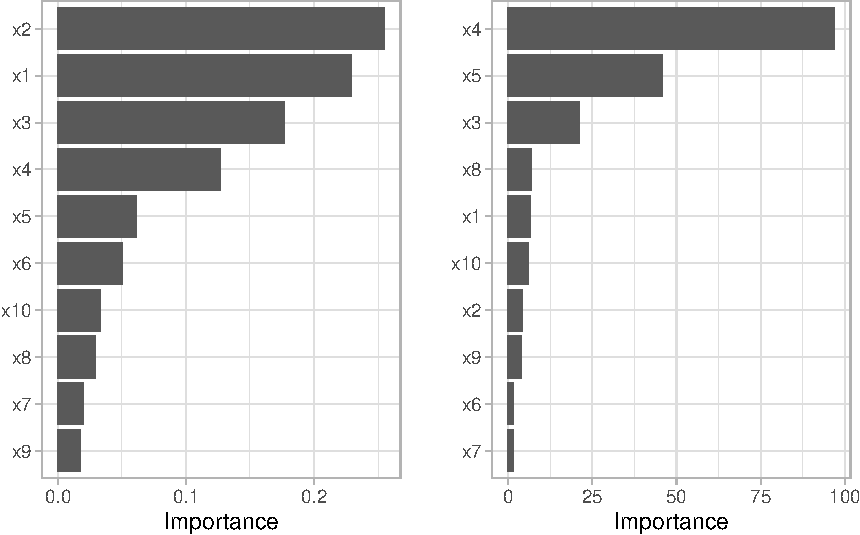
\includegraphics[width=0.7\linewidth]{greenwell-boehmke_files/figure-latex/vip-nnet-1} 

}

\caption[Example VIPs from a single-hidden-layer NN fit to the simulated Friedman data]{Example VIPs from a single-hidden-layer NN fit to the simulated Friedman data.}\label{fig:vip-nnet}
\end{figure}
\end{Schunk}

\section{Model-agnostic VI}

Model-agnostic interpredibility separates interpretation from the model.
Compared to model-specific approaches, model-agnostic VI methods are
more flexible and can be applied to any supervised learning algorithm.
In this section, we discuss model-agnostic methods for quantifying
global feature importance using three different approaches: 1) partial
dependence plots (PDPs), 2) \dfn{individual conditional expectation}
(ICE) curves, and 3) permutation-based feature importance. For specific
details on approaches 1)--2), see \citet{greenwell-simple-2018}.

\subsection{PDP method}

Our first model-agnostic approach is based on quantifying the
``flatness'' of the PDPs of each feature. PDPs help visualize the effect
of low cardinality subsets of the feature space on the estimated
prediction surface (e.g., main effects and two/three-way interaction
effects.). PDPs provide model-agnostic interpretations and can be
constructed in the same way for any supervised learning algorithm; for
an overview, see \citet{greenwell-pdp-2017}. Below, we fit a projection
pursuit regression (PPR) model and construct PDPs for each feature using
the \CRANpkg{pdp} package \citet{greenwell-pdp-2017}. The results are
displayed in Figure\textasciitilde{}\ref{fig:pdp-ppr}. Notice how the
PDPs for the uninformative features are relatively flat compared to the
PDPs for features \code{x1}--\code{x2}!

\begin{Schunk}
\begin{Sinput}
# Load required packages
library(pdp)

# Fit a PPR model (nterms was chosen using the caret package with 5 repeats of 
# 5-fold cross-validation)
pp <- ppr(y ~ ., data = trn, nterms = 11)  

# PDPs for all 10 features
features <- paste0("x", 1:10)
pdps <- lapply(features, FUN = function(feature) {
  pd <- partial(pp, pred.var = feature)
  autoplot(pd) + 
    ylim(range(trn$y)) + 
    theme_light()
})
grid.arrange(grobs = pdps, ncol = 5)
\end{Sinput}
\begin{figure}

{\centering 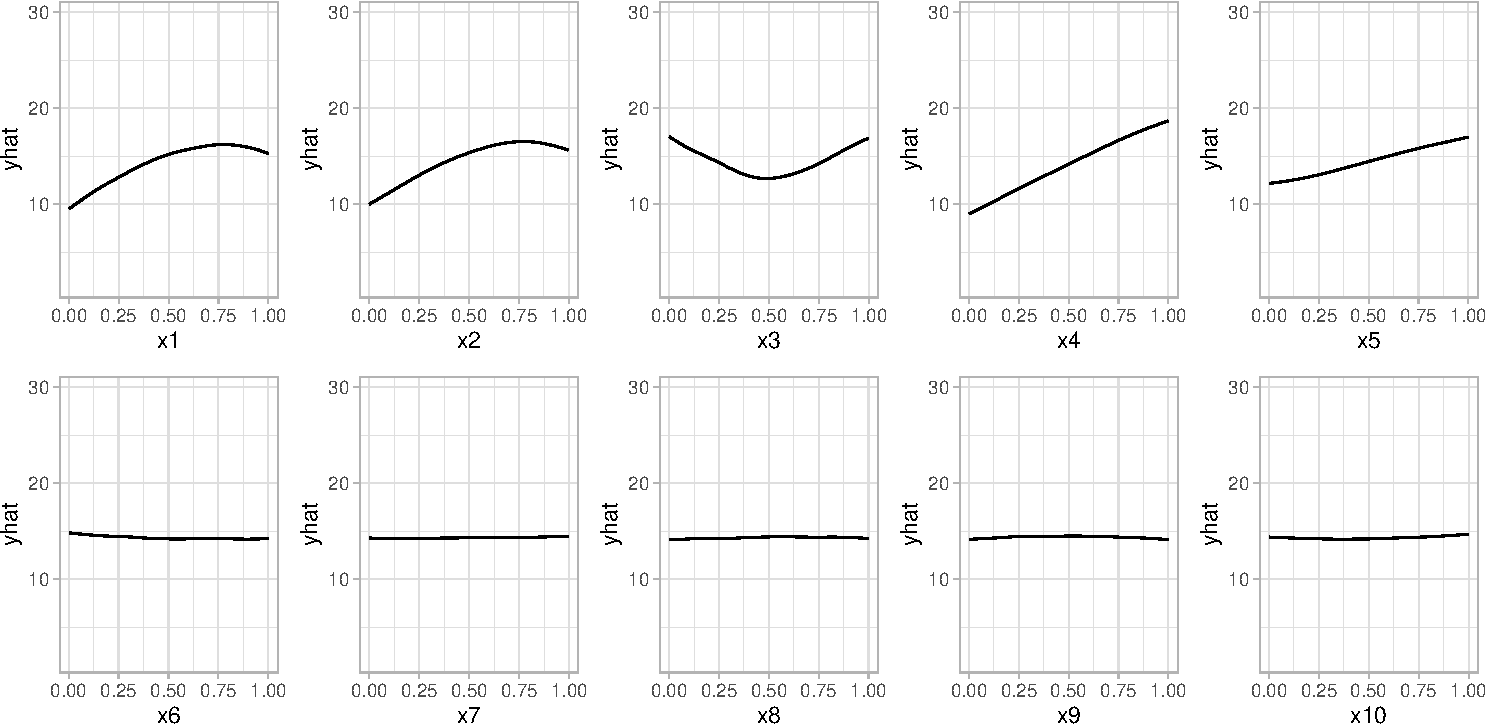
\includegraphics[width=1\linewidth]{greenwell-boehmke_files/figure-latex/pdp-ppr-1} 

}

\caption[PDPs of main effects in the PPR model fit to the simulated Friedman data]{PDPs of main effects in the PPR model fit to the simulated Friedman data.}\label{fig:pdp-ppr}
\end{figure}
\end{Schunk}

Next, we compute PDP-based VI scores for the PPR and NN models. The PDP
method constructs VI scores that quantify the relative ``flatness'' of
each PDP (by default, this is defined by computing the standard
deviation of the \(y\)-axis values for each PDP). To use the PDP method,
specify \code{method = "pdp"} in the call to \code{vi()} or
\code{vip()}:

\begin{Schunk}
\begin{Sinput}
# Fit a PPR model (nterms was chosen using the caret package with 5 repeats of 
# 5-fold cross-validation)
pp <- ppr(y ~ ., data = trn, nterms = 11)  

# Plot VI scores
p1 <- vip(pp, method = "pdp") + ggtitle("PPR")
p2 <- vip(nn, method = "pdp") + ggtitle("NN")

# Figure 7
grid.arrange(p1, p2, ncol = 2)
\end{Sinput}
\begin{figure}

{\centering 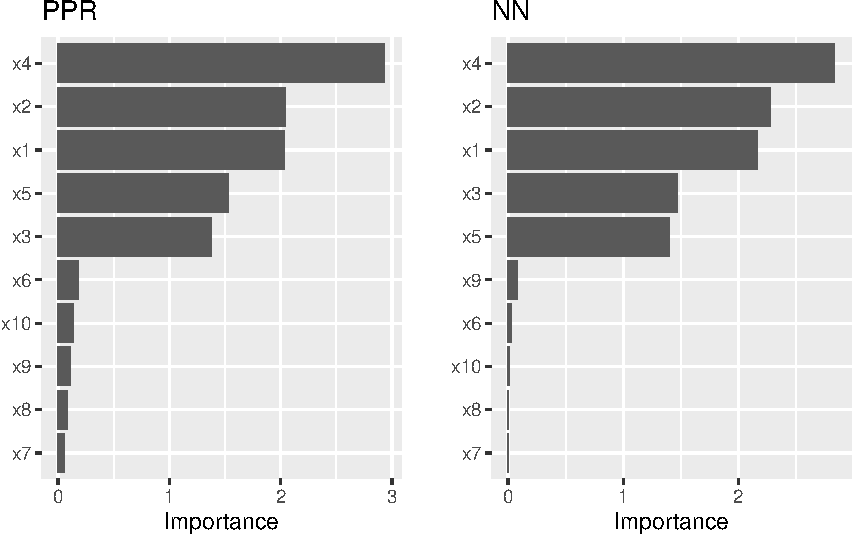
\includegraphics[width=0.7\linewidth]{greenwell-boehmke_files/figure-latex/pdp-ppr-nn-1} 

}

\caption[PDP-based feature importance for the PPR and NN models fit to the simulated Friedman data]{PDP-based feature importance for the PPR and NN models fit to the simulated Friedman data.}\label{fig:pdp-ppr-nn}
\end{figure}
\end{Schunk}

In Figure\textasciitilde{}\ref{fig:pdp-ppr-nn} we display the PDP-based
feature importance for the previously obtained PPR and NN models. These
VI scores essentially capture the variability in the partial dependence
values for each main effect.

\subsection{ICE curve method}

The ICE curve method is similar to the PDP method. The only difference
is that we measure the ``flatness'' of each ICE curve and then aggregate
the results (e.g., by averaging). If there are no (substantial)
interaction effects, using \code{method = "ice"} will produce results
similar to using \code{method = "pdp"}. However, if strong interaction
effects are present, they can obfuscate the main effects and render the
PDP-based approach less useful (since the PDPs for important features
can be relatively flat when certain interactions are present; see
\citet{goldstein-peeking-2015} for details). In fact, it is probably
safest to always use \code{method = "ice"}.

Below, we display the ICE curves for each feature in the PPR model using
the same \(y\)-axis scale; see Figure\textasciitilde{}\ref{fig:ice-ppr}.
Again, there is a clear difference between the ICE curves for features
\code{x1}--\code{x5} and \code{x6}--\code{x10}; the later being
relatively flat by comparison. Also, notice how the ICE curves within
each feature are relatively parallel (if the ICE curves within each
feature were perfectly parallel, the standard deviation for each curve
would be the same and the results will be identical to the PDP method).
In this example, the interaction term between \code{x1} and \code{x2}
does not obfuscate the PDPs for the main effects and the results are not
much different.

\begin{Schunk}
\begin{Sinput}
# ICE curves for all 10 features
ice_curves <- lapply(features, FUN = function(feature) {
  ice <- partial(pp, pred.var = feature, ice = TRUE)
  autoplot(ice, alpha = 0.1) +
    ylim(range(trn$y)) +
    theme_light()
})

# Figure 8
grid.arrange(grobs = ice_curves, ncol = 5)
\end{Sinput}
\begin{figure}

{\centering 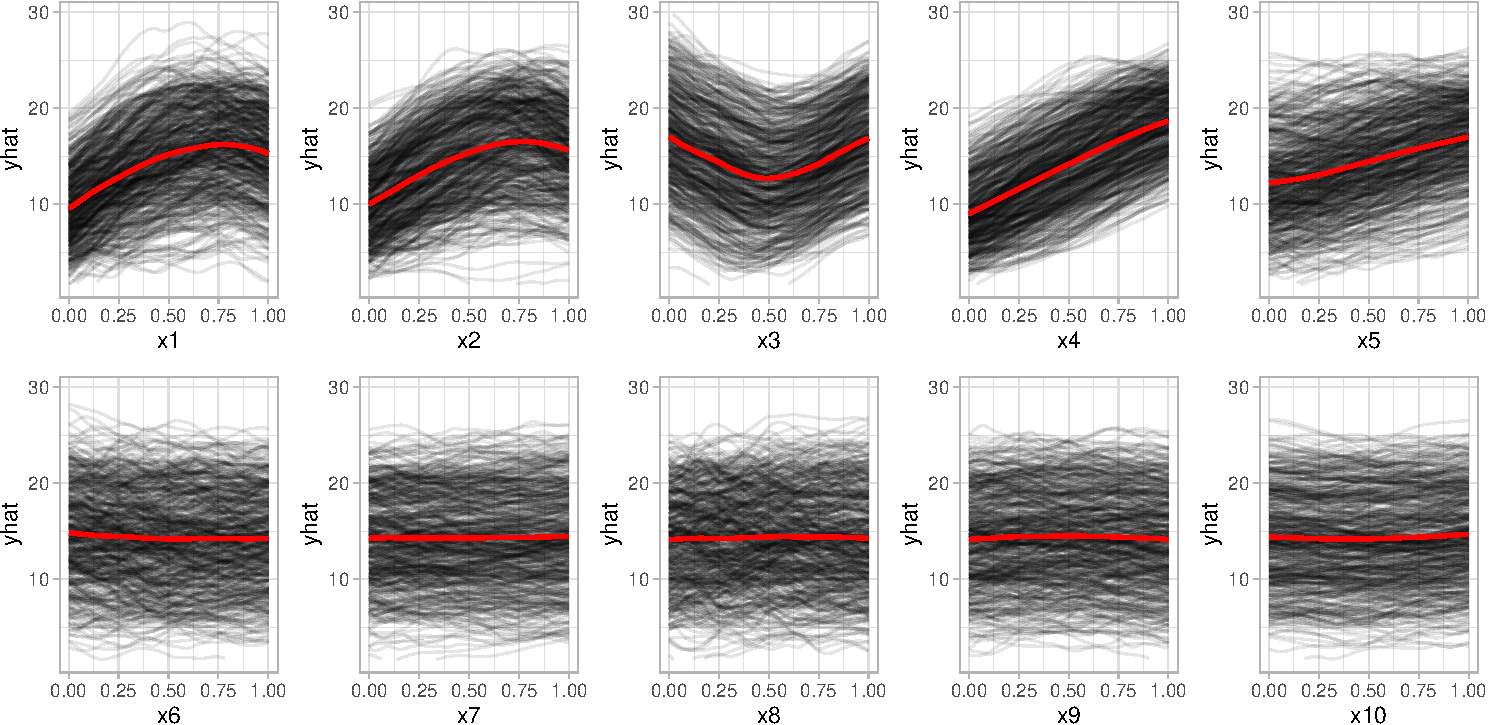
\includegraphics[width=1\linewidth]{greenwell-boehmke_files/figure-latex/ice-ppr-1} 

}

\caption[ICE curves for each feature in the PPR model fit to the simulated Friedman data]{ICE curves for each feature in the PPR model fit to the simulated Friedman data. The red curve represents the PDP (i.e., the averaged ICE curves).}\label{fig:ice-ppr}
\end{figure}
\end{Schunk}

Obtaining the ICE-based feature importance scores is also
straightforward, just specify \code{method = "ice"} in the call to
\code{vip::vi()} or \code{vip::vip()}. This is illustrated in the code
chunk below and the results are
Figure\textasciitilde{}\ref{fig:vip-ice-ppr-nn} are similar to those
obtained using the PDP method.

\begin{Schunk}
\begin{Sinput}
# Plot VI scores
p1 <- vip(pp, method = "ice") + ggtitle("PPR")
p2 <- vip(nn, method = "ice") + ggtitle("NN")

# Figure 9
grid.arrange(p1, p2, ncol = 2)
\end{Sinput}
\begin{figure}

{\centering 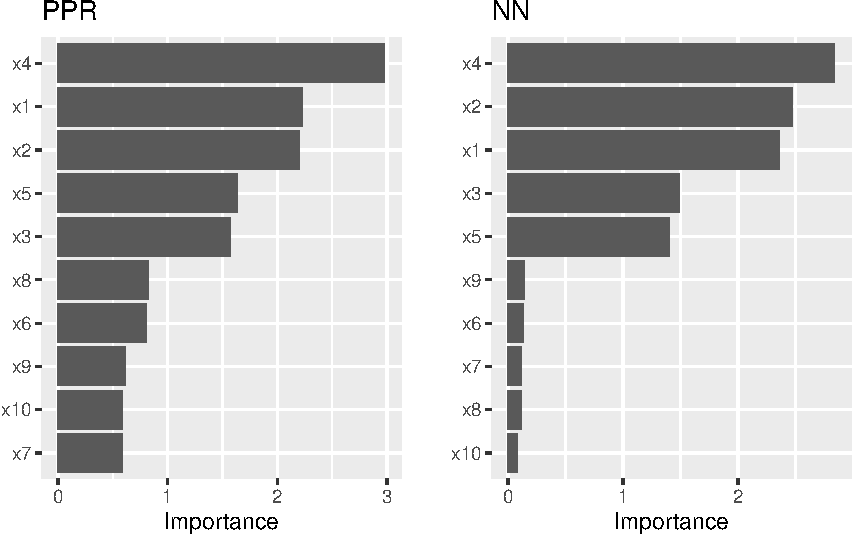
\includegraphics[width=0.7\linewidth]{greenwell-boehmke_files/figure-latex/vip-ice-ppr-nn-1} 

}

\caption[ICE-based feature importance for the PPR and NN models fit to the simulated Friedman data]{ICE-based feature importance for the PPR and NN models fit to the simulated Friedman data.}\label{fig:vip-ice-ppr-nn}
\end{figure}
\end{Schunk}

When using \code{method = "pdp"} or \code{method = "ice"}, the feature
effect values are stored as attributes \code{"pdp"} and \code{"ice"},
respectively. This is a convenience so that the feature effect plots
(e.g., PDPs and ICE curves) can easily be reconstructed and compared
with the VI scores, as demonstrated in the example below (see
Figure\textasciitilde{}\ref{fig:pdp-from-attr}):

\begin{Schunk}
\begin{Sinput}
# Construct PDP-based variable importance scores
(vis <- vi(pp, method = "pdp"))
\end{Sinput}
\begin{Soutput}
#> # A tibble: 10 x 2
#>    Variable Importance
#>    <chr>         <dbl>
#>  1 x4           2.93  
#>  2 x2           2.05  
#>  3 x1           2.04  
#>  4 x5           1.53  
#>  5 x3           1.38  
#>  6 x6           0.183 
#>  7 x10          0.139 
#>  8 x9           0.113 
#>  9 x8           0.0899
#> 10 x7           0.0558
\end{Soutput}
\begin{Sinput}
# Reconstruct PDPs for all 10 features
par(mfrow = c(2, 5))
for (name in paste0("x", 1:10)) {
  plot(attr(vis, which = "pdp")[[name]], type = "l", ylim = c(9, 19), las = 1)
}
\end{Sinput}
\begin{figure}

{\centering 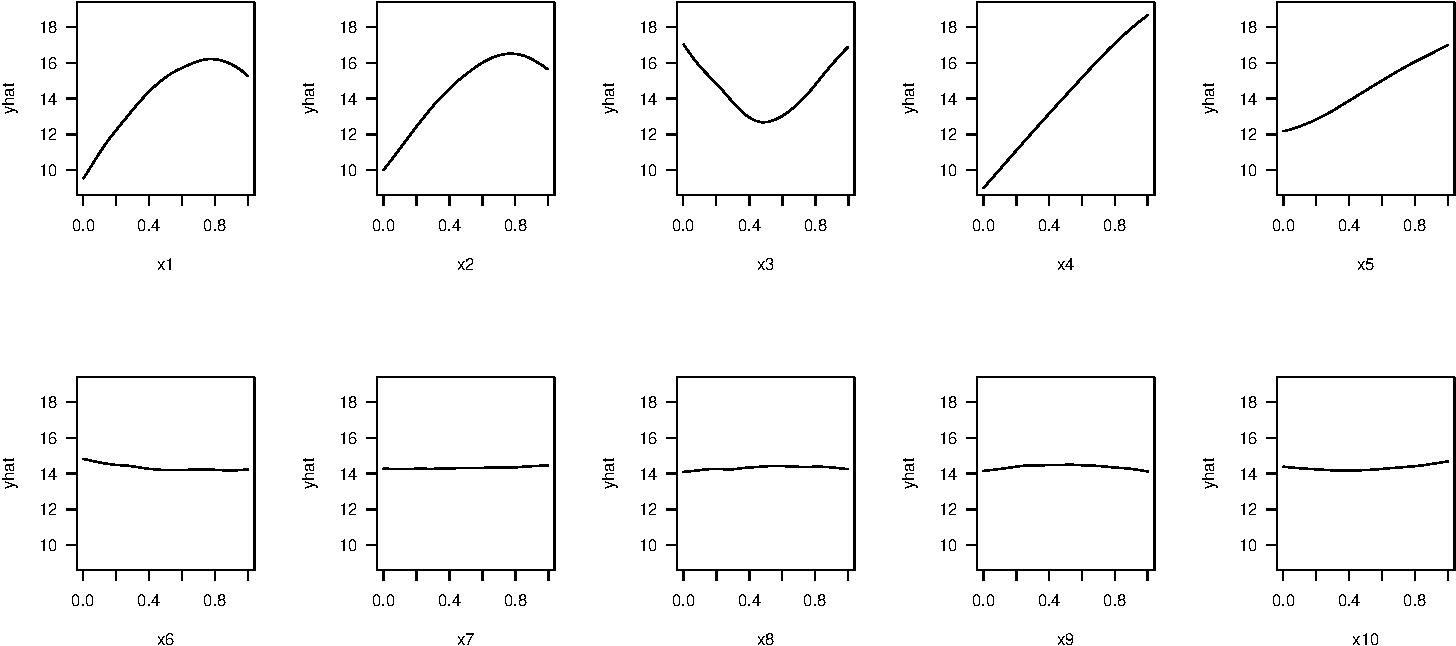
\includegraphics[width=1\linewidth]{greenwell-boehmke_files/figure-latex/pdp-from-attr-1} 

}

\caption[PDPs for all ten features reconstructed from the \code{pdp} attribute of the \code{vis} object]{PDPs for all ten features reconstructed from the \code{pdp} attribute of the \code{vis} object.}\label{fig:pdp-from-attr}
\end{figure}
\end{Schunk}

\subsection{Permutation method}

\begin{algorithm}
\begin{enumerate}
  \item For $i = 1, 2, \dots, j$:
  \begin{enumerate}
    \item Permute the values of feature $X_i$ in the training data.
    \item Recompute the performance metric on the permuted data $\mathcal{M}_{perm}$.
    \item Record the difference from baseline using $imp\left(X_i\right) = \mathcal{M}_{perm} - \mathcal{M}_{orig}$.
  \end{enumerate}
  \item Return the VI scores $imp\left(X_1\right), imp\left(X_2\right), \dots, imp\left(X_j\right)$.
\end{enumerate}
<!-- \caption{A simple algorithm for constructing permutation-based VI scores. \label{alg:permute}} -->
\end{algorithm}

--\textgreater{} --\textgreater{} --\textgreater{} --\textgreater{}
--\textgreater{} --\textgreater{}

--\textgreater{} --\textgreater{} --\textgreater{} --\textgreater{}
--\textgreater{} --\textgreater{}

--\textgreater{} --\textgreater{} --\textgreater{} --\textgreater{}
--\textgreater{} --\textgreater{}

--\textgreater{} --\textgreater{} --\textgreater{} --\textgreater{}
--\textgreater{} --\textgreater{}

--\textgreater{} --\textgreater{} --\textgreater{} --\textgreater{}
--\textgreater{} --\textgreater{}

\subsection{Shapley method}

Starting with \pkg{vip} 0.1.4 you can now construct VI scores based on
\dfn{Shapley values} REF. Suppose we make a prediction for an
observation \(x\prime\), denoted \(f\left(x\prime\right)\). The Shapley
values for \(f\left(x\prime\right)\)\ldots{}

--\textgreater{} --\textgreater{} --\textgreater{} --\textgreater{}
--\textgreater{} --\textgreater{}

--\textgreater{} --\textgreater{} --\textgreater{} --\textgreater{}
--\textgreater{} --\textgreater{}

\section{Acknowledgments}

\bibliography{greenwell-boehmke}


\address{%
Brandon M. Greenwell\\
University of Cincinnati\\
2925 Campus Green Dr\\ Cincinnati, OH 45221\\ United States of America\\ ORCiD---\href{https://orcid.org/0000-0002-8120-0084}{0000-0002-8120-0084}\\
}
\href{mailto:greenwell.brandon@gmail.com}{\nolinkurl{greenwell.brandon@gmail.com}}

\address{%
Bradley C. Boehmke\\
University of Cincinnati\\
2925 Campus Green Dr\\ Cincinnati, OH 45221\\ United States of America\\ ORCiD---\href{https://orcid.org/0000-0002-3611-8516}{0000-0002-3611-8516}\\
}
\href{mailto:bradleyboehmke@gmail.com}{\nolinkurl{bradleyboehmke@gmail.com}}

